% This is samplepaper.tex, a sample chapter demonstrating the
% LLNCS macro package for Springer Computer Science proceedings;
% Version 2.20 of 2017/10/04
%
\documentclass[runningheads]{llncs}
%
\usepackage{graphicx}
\usepackage{amsmath}
\usepackage{todonotes}
\usepackage{biblatex}
\addbibresource{bibliography.bib}
% Used for displaying a sample figure. If possible, figure files should
% be included in EPS format.
%
% If you use the hyperref package, please uncomment the following line
% to display URLs in blue roman font according to Springer's eBook style:
% \renewcommand\UrlFont{\color{blue}\rmfamily}

\begin{document}
%
\title{Early-stage nodule generation with deep image prior}
%
%\titlerunning{Abbreviated paper title}
% If the paper title is too long for the running head, you can set
% an abbreviated paper title here
%
\author{Octavio E. Martinez Manzanera\inst{1} \and
Vasileios Baltatzis\inst{1} \and
Sujal Desai\inst{2,3} \and
Anand Devaraj\inst{2} \and
Sam Ellis\inst{1} \and
Loic Le Folgoc\inst{3} \and
Arjun Nair\inst{4} \and
Ben Glocker\inst{3} \and
Julia Schnabel\inst{1}}
%
\authorrunning{O.E. Martinez Manzanera et al.}
% First names are abbreviated in the running head.
% If there are more than two authors, 'et al.' is used.
%
\institute{Biomedical Engineering and Imaging Sciences, King’s College London, UK \and
The Royal Brompton & Harefield NHS Foundation Trust, London UK \and
BioMedIA, Imperial College London, UK \and
Department of Radiology, University College London, UK}
%
\maketitle              % typeset the header of the contribution
%
\begin{abstract}
The presence of lung nodules is the key feature of lung cancer diagnosis. They are commonly identified  by an experienced radiologist in a computer tomography (CT) scan. In recent years, different Convolutional Neural Network (CNN) architectures have been proposed to support this diagnosis. However, both radiologists and CNNs can only identify nodules that are already formed or at least have a recognizable structure. This can leave out early-stage nodules which are fundamental in the detection of early-stage lung cancer. In this study we apply the deep image prior inpainting technique to CT lung slices . We applied this technique to 800 CT scans from the Lung Image Database Consortium (LIDC) dataset. Specifically, we masked out the lung nodules using the union of the segmentations masks provided by a maximum of four annotators. We expect that the generated dataset contains the anatomical characteristics of the lungs before the nodules appearance. Once the generated dataset was obtained we employed a generative model (cycleGAN) to produce images that represent the nodules' evolution. Both the generated dataset using deep image prior and the images showing nodule progression were qualitatively assessed by experienced radiologists. Results XX. We expect that this technique and the obtained dataset could aid the understanding of nodule progression in lung cancer and improve early-stage detection.

\keywords{Lung cancer  \and Deep image prior \and Computed Tomography}
\end{abstract}
%
%
%
\section{Introduction}

Among all types of cancer, lung cancer is the one with highest mortality rates and the second in incidence among men and women \cite{doi:10.3322/caac.21551}. Its diagnosis is usually performed in two steps, first, pulmonary nodules are detected and then they are characterized. Therefore, nodules are identified only once they have grown sufficiently to be recognizable by a radiologist. The consequence is that cancer is usually diagnosed at later stages when treatment options are already limited.
Commonly, physicians request imaging studies when patients present specific symptoms that might be related to lesions or anomalies in an organ. This is the case of nodules in lung cancer. There is however, a minority of cases of incidental nodules identified on screening studies or during an evaluation requested for other medical reasons. Therefore, the identification of early-stage nodules is considerably less frequent than the one of XX. Moreover, the knowledge about their structure and emergence is scarce. This is a strong limitation that hinders the early diagnosis of lung cancer.

The LIDC is a dataset composed of 1018 cases of computed tomography (CT scans) ~\cite{pmid21452728}. In this dataset four thoracic radiologists reviewed each scan and provided a segmentation around each lesion identified. A total of 2669 nodules >= 3 mm where identified by at least one radiologist. 

Inpainting with deep image prior allows the reconstruction of images with areas that are blanked out using a Convolutional Neural Network (CNN). This technique does not require a pretrained network, therefore it can be applied to images individually to avoid introducing external features into an image. Deep image prior utilizes contextual features from the image in question and interpolates the unknown regions with relevant textures from the image\cite{DBLP:journals/corr/abs-1711-10925}. 

\section{Methods}
\subsection{Preprocessing}
We converted all scans to Hounsfield units and resampled them to an isomorphic resolution. We discarded those scans that XX. This resulted in a dataset of XX scans. We focused this analysis on the corresponding middle slice of each nodule. We employed the pylidc library~\cite{pylidc} and custom scripts for data preprocessing. Individual nodule segmentations might not be completely accurate and might leave out parts of the nodule. Therefore, for each nodule we employed the union of all available segmentations to produce a slightly larger mask. Then, we dilate a single time this area to produce a mask that encompass the whole nodule. The inputs to the inpainting CNN were the slice at the center of the nodule and its corresponding mask where the region outside of the lungs and the dilated area of the nodule is occluded (Fig.~\ref{fig1}).

\begin{figure}
\includegraphics[width=\textwidth]{inpainting-difference-caption.png}
\caption{Images A and B are the original slice and the inpainted slice. Image C is the mask employed for inpainting where the pixels from the nodule and the pixels outside the lungs are blanked out. Image D is the absolute difference of images A and B. Images E and F are a detailed view of the original and inpainted images. It can be observed that image F contains almost all details from image E except the nodule. Image H shows a detailed version of the pixels' differences. Finally, image G shows the pixel intensity distribution of the pixels belonging to the nodule mask of the original image (cyan) and the inpainted version (red). It is important to remark that the scale of the images showing differences (D and H) is considerably smaller [0 - 0.03] than the scale of the other images [0 - 1].} \label{fig1}
\end{figure}

\subsection{Deep image Prior}
In their original study, Ulyanov et al~\cite{DBLP:journals/corr/abs-1711-10925} defined the reconstruction of a partially occluded image with the optimization problem described in (1), where, \(x_o\) represents the partially occluded image, \(z\) represents an image filled in with random noise, \(f_\theta\) represents a deep CNN parameterized by \(\theta\), \(m\) represents the binary mask \(m = \in \{0, 1\}^{HxW} \) and \(\odot\) is Hadamard's product. For our case, the mask indicates that the loss function should only consider those pixels inside the lungs but not the pixels inside the nodule. 
\begin{equation}
\textrm{min}_\theta  \|(f_\theta(z) - x_0) \odot m) \|^2
\end{equation}

 We minimized the mean squared error (MSE) for all the pixels according to the mask. This way, the network will try to reproduce the original image and it will fill in the occluded areas with relevant information obtained from the rest of the regions inside the lungs. We employed an encoder - decoder architecture similar to ~\cite{DBLP:journals/corr/abs-1711-10925} without skip connections and with five downsampling blocks. Each block was composed of three consecutive Convolutional, Batch-normalization and Leaky ReLU operations.

For each image, before minimizing the MSE we found an adequate learning rate (LR) using a similar technique described to the one described in~\cite{DBLP:journals/corr/Smith15a}. We automate the LR selection finding the longest, continuous negative slope in the LR finder plot (Fig.~\ref{fig2}) and selecting a LR close to the end of the slope.  Once the LR was identified we trained our CNN for 10,000 iterations. We employed learning rate annealing and we saved the best results according to the minimum MSE. We employed early stopping after 500 iterations of no further improvement. For those images which completed 10,000 training iterations, the average computing time was six minutes using a Titan-X GPU. Even when the reconstructions achieved a low MSE there is no guarantee that the nodule mask region is successfully filled in with relevant lung-like features and does not resemble a nodule. Two co-authors qualitatively analyzed the inpainted images to determine whether the nodule in question was still present in the inpainted images. The results of the qualitative evaluation were employed to define a metric to quantify the degree to which nodules were succesfully inpainted with a lung-like texture. We employed the results of the qualitative assessment as target labels and three inpainting features in a logistic regression model. The features employed were the difference between the mean intensity of the pixels in the nodule mask of the original image and the corresponding pixels of the inpainted image, the intensity of the pixels in the nodule mask of the inpainted image and the nodule size. The first two features come from the rationale that areas without nodule are generally of lower intensity than areas where nodules are located.

\begin{figure}
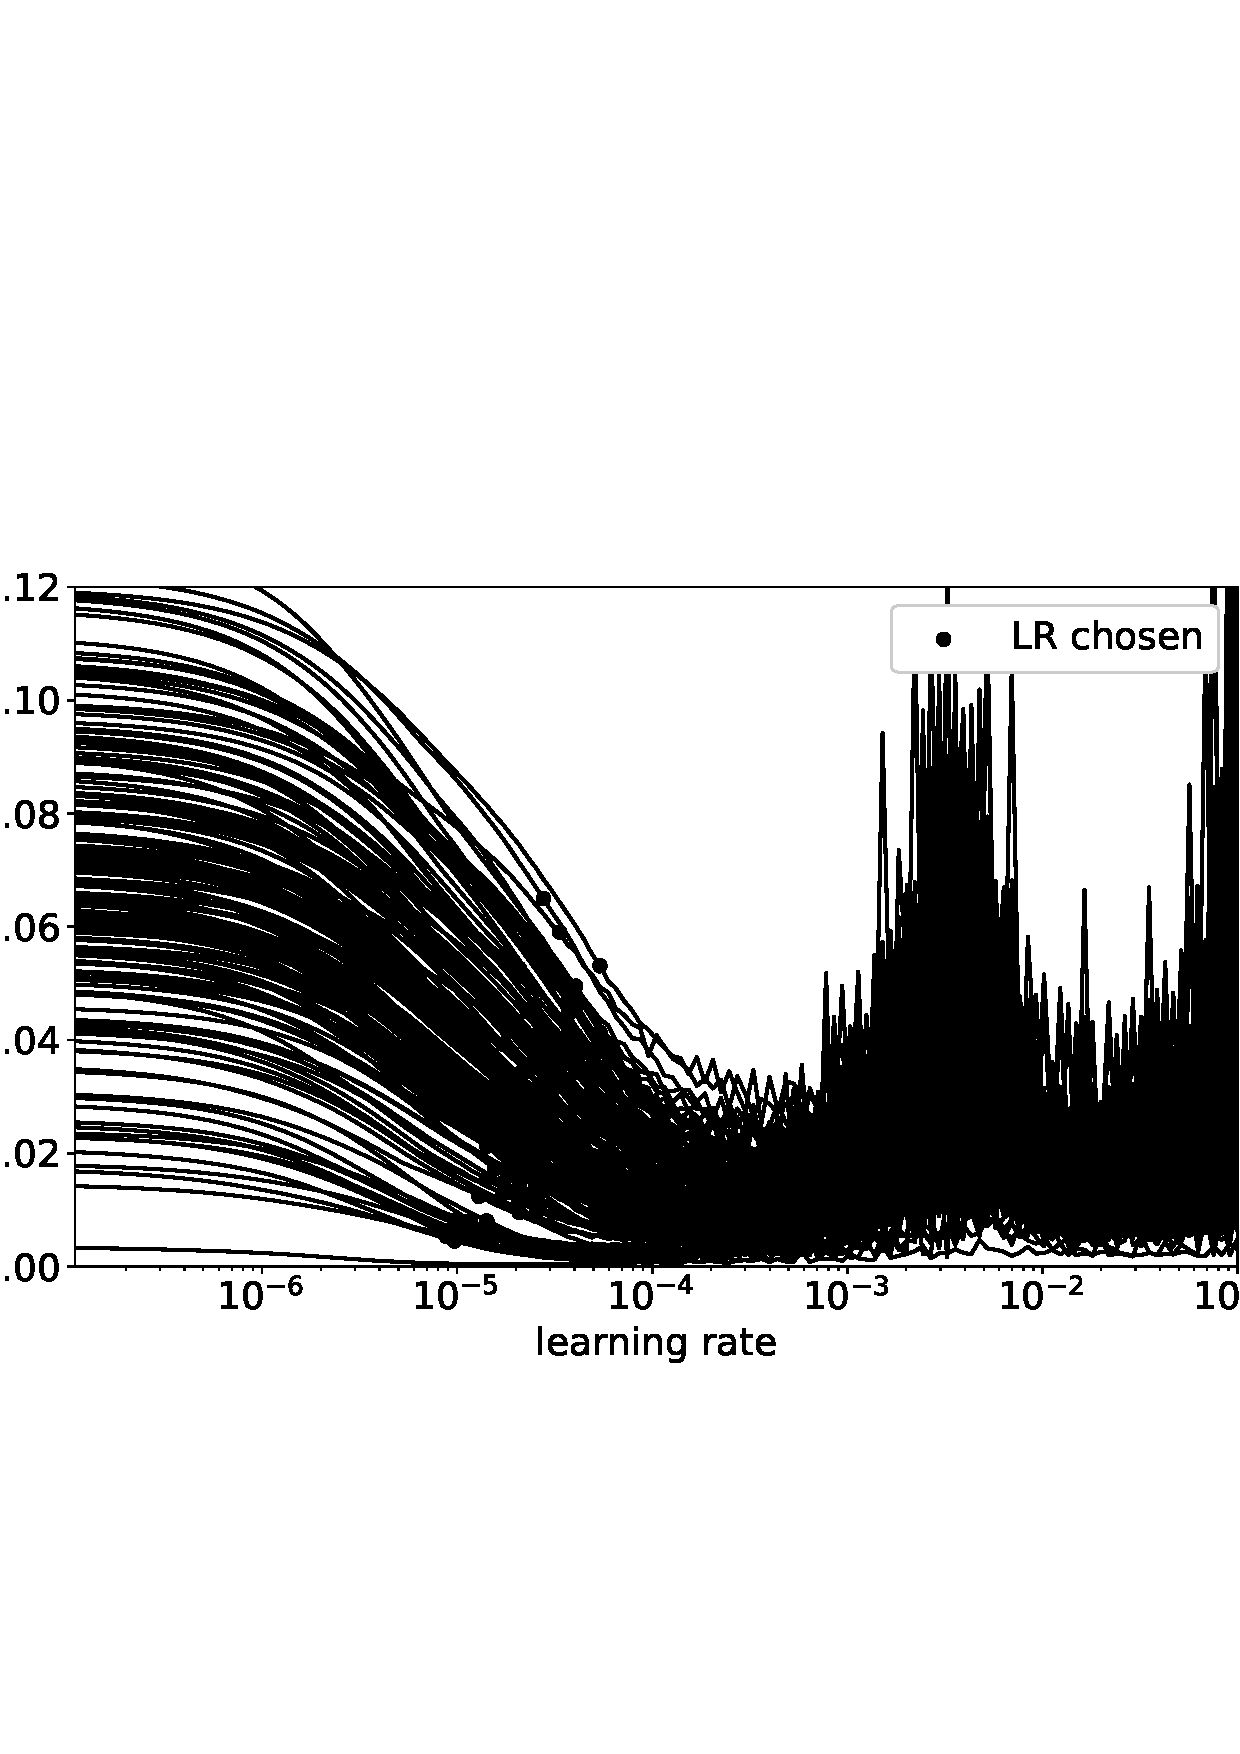
\includegraphics[width=\textwidth]{learning-rate.png}
\caption{Left: LR finder plots for a subset of images. Each line describes the inpainting loss for one iteration at different learning rates. Low LRs (left) show very small differences and high LR (right) show instability. Adequate LR are found in the region with steepest negative slope (large loss reduction per iteration).  } \label{fig2}
\end{figure}

\subsection{cycleGAN}
We employed the subset of successfully inpainted images according to the nodules' pixel intensity mean difference to construct a dataset of (nodule and inpainted) paired images. We trained a cycleGAN~\cite{CycleGAN2017} based with this dataset to simulate the development and growth of nodules and also to obtain a tool that can produce the opposite effect. The cycleGAN is composed of two generators, the first generator \(G\) maps the images from the source domain \(X\) to the target domain \(Y\) (\(G: X \rightarrow Y\)) and the second generator \(F\) performs the mapping in the other direction (\(F: Y \rightarrow X\)). The cycleGAN loss is composed of  various components. The cycle-consistency loss enforces that mapping an image from one domain to the second domain and back \(X \rightarrow Y \rightarrow X\) should produce an image similar to the original one (Eq. 2). The adversarial loss tries to match the distribution of generated images to the one of the target domain (Eq. 3). \todo[color=green!40]{mention identity loss and mask applyied in GAN}. The generators were composed of nine residual blocks where the non-identity path contained convolution operations, instance normalization and a ReLU activation~\cite{CycleGAN2017}. Similarly to the inpainting technique (and to the patchGAN XX) we added a binary mask to the cycleGAN loss to focus on the pixels inside the lungs (eq. XX). We trained the cycleGAN for 200 epochs with a LR = 0.0002. 

\begin{equation}
\begin{aligned}
\mathcal{L}_{GAN}(G, D_Y, X, Y) = \mathbb{E}_{y~\mathbb{P}_{data}(y)} [log D_Y(y)] + \\
\mathbb{E}_{x~\mathbb{P}_{data}(x)} [log(1 - D_Y(G(x))]\\
\end{aligned}
\end{equation}
\begin{equation}
\begin{aligned}
\mathcal{L}_{GAN}(G, D_X, X, Y) = \mathbb{E}_{x~\mathbb{P}_{data}(x)} [log D_X(y)] + \\
\mathbb{E}_{y~\mathbb{P}_{data}(y)} [log(1 - D_X(G(y))]\\
\end{aligned}
\end{equation}
\begin{equation}
\begin{aligned}
\mathcal{L}_{cyc}(G, F) = \mathbb{E}_{x~\mathbb{P}_{data}(x)} [\|F(G(x)) - x\|_1] + \\
\mathbb{E}_{y~\mathbb{P}_{data}(y)} [\|G(F(y)) - y\|_1]
\end{aligned}
\end{equation}

\section{Results}
\subsection{Deep image prior}
We performed inpainting with deep image prior on 2,324 slices. Inpainting achieved a MSE error of 2.7e-4 (1.0e-3). The qualitative assessment of successfully inpainted nodules selected 819 images (35.2\%) (Fig.~\ref{fig3}). The results of the logistic regression model using the labels produced by the qualitative assessment can be seen on Table~\ref{tab1}.

\begin{figure}
\includegraphics[width=\textwidth]{inpainting-examples.png}
\caption{Images selected in the qualitative assessment. For each image pair the left image shows the region where the nodule is located and the image on the right same shows the same region but the nodule area is now inpainted with lung-like texture.} \label{fig3}
\end{figure}

\begin{table}
\caption{Logistic regression results.}\label{tab1}
\begin{tabular}{|l|l|l|}
\hline
Features &  \beta & p-value\\
\hline
Intensity difference & 1.27 & \(<\)0.01\\
Intensity inpainted & -1.93 & \(<\)0.01\\
Nodule area & -0.08 & 0.02\\
\hline
\end{tabular}
\end{table}

 \todo[color=green!40]{Mention the characteristics of successful inpainting: e.g. according to the qualitatively assessment, XX\% were smaller than, XX\% corresponded to GGN nodules}

\subsection{cycleGAN}
The images generated by one of the cycleGAN generators can be seen in Fig.~\ref{fig4}. We observed that for most cases the images generated by the nodule generator presented a general pattern where nodules grew in size and intensity. However, it is important to remark that this pattern was not constant and for some epochs size and intensity decreased.

\begin{figure}
\includegraphics[width=\textwidth]{cycleGAN-nodule-generator-v6.png}
\caption{Nodules generation using cycleGAN. Five training examples of nodule generation using cycleGAN are shown. For each row, the image on the right is the original image with one nodule depicted inside an orange rectangle. The image on the left is the inpainted version of the image on the right. We can observe that the nodule is not visible. The images in the middle, represent, from left to right the nodule growth across various epochs using one generator from cycleGAN.} \label{fig4}
\end{figure}

\section{Discussion}
\subsection{Deep image prior}
In this study we employed inpainting with deep image prior in images with lung nodules to generate similar images without such nodules. Then, we employed a cycleGAN to produce images that represent the development of lung nodules. From a qualitative point of view, deep image prior produced a good image without the nodule for approximately 1/3 of the images. However, this assessment should be replicated by an experienced radiologist and more information from the lungs should be provided to the network. 
There are several points that can be improved in order to obtain a better inpainting performance qualitatively and in terms of MSE. Firstly, inpainting should be performed in a 3D fashion using 3D CNNs and using the complete information, or as most as possible, from the regions inside the lungs in the CT scan. The current 2D approach limits the lung information to the information in one slice. We observed that pixels with relative high intensity next to the nodules (e.g. from vessels) can influence the inpainting process. We expect that inpainting with a 3D volume would allow the network to identify when a nodule is in contact with a vessel or a structure placed in a transversal direction, a feature that is not possible with a 2D slice. We performed preliminary experiments with this technique, but memory and computing time constrains prevented us from completing the experiments. Secondly, the selection an optimal inpainting CNN architecture should be explored. In preliminary experiments we evaluated UNet architectures but their performance, similarly to the results reported in ~\cite{DBLP:journals/corr/abs-1711-10925}, were generally lower than the ones of encoder-decoder architectures. We deem valuable studying deeper architectures, especially for those images that do not achieve good inpainting results. Having said this, we believe that 3D architectures will lead to better results, qualitatively and in terms of MSE.

\subsection{cycleGAN}
Both generators in cycleGAN produce acceptable intermediate results. 
In previous years a wide variety of generative models has emerged. We consider that cycleGAN has the potential of providing good performance in both generation tasks, nodule progression and nodule image removal. However, other generative models should also be explored to, for instance, observe the possible progression of a specific types of nodule (ground glass) from a nodule candidate. 

We believe that the combination of deep image prior and generative models can lead to a better understanding of nodule progression and to create tools that improve the detection and identification of early-stage nodules. Moreover, we believe that deep image prior offers other applications of potential clinical value. For instance, the features generated and employed to fill in occluded regions might be valuable for identification of malignant cases even before nodules can be visually identified by experienced radiologists.
%
% ---- Bibliography ----
%
% BibTeX users should specify bibliography style 'splncs04'.
% References will then be sorted and formatted in the correct style.
%
% \bibliographystyle{splncs04}
% \bibliography{mybibliography}
%

\printbibliography
\end{document}
